% ------------------------------------------------------------------------------------------------
% Journal of Intelligent Manufacturing
% Ver. 3.1 -- Adding some result figures
% ------------------------------------------------------------------------------------------------

\PassOptionsToPackage{hypertexnames=false}{hyperref}
\documentclass[sn-basic]{sn-jnl} % Basic Springer Nature Reference Style

%% Standard Packages
\usepackage{caption}
\usepackage{subcaption}
\usepackage{graphicx}%
\usepackage{pgfplots}
\pgfplotsset{compat=1.18}
\usepackage{multirow}%
\usepackage{amsmath,amssymb,amsfonts}%
\usepackage{amsthm}%
\usepackage{mathrsfs}%
\usepackage[title]{appendix}%
\usepackage{textcomp}%
\usepackage{manyfoot}%
\usepackage{setspace}
\usepackage[table]{xcolor}
\usepackage{booktabs}

% (Removed algorithmic packages; pseudocode moved to Appendix listings.)

% --- MACRO DEFINITION ---
\newcommand{\faintcmidrule}[1]{%
	\arrayrulecolor{black!30}%
	\cmidrule{#1}%
	\arrayrulecolor{black}%
}

% % % Usage: \faintcmidrule{2-4} % Optional thickness: \faintcmidrule[0.2pt]{2-4}
% \newcommand{\faintcmidrule}[2][0.25pt]{%
%   \cmidrule[#1](lr){#2}%
% }

\graphicspath{{figures/}}

% Avoid large bookmark-level jumps when using \paragraph headings.
% (hyperref warns when jumping from \subsection directly to \paragraph.)
\makeatletter
\def\toclevel@paragraph{3}
\def\toclevel@subparagraph{4}
\makeatother

\onehalfspacing
% \lstset{
%         basicstyle=\ttfamily\footnotesize,
%         columns=fullflexible,
%         breaklines=true,
%         frame=single,
%         xleftmargin=0.5em,
%         xrightmargin=0.5em,
%         aboveskip=0.8em,
%         belowskip=0.8em
% }

\begin{document}

\title[Lightweight RL for Edge PdM]{Lightweight Reinforcement Learning for Edge Predictive Maintenance: \textsc{REINFORCE} with Attention for Milling Tool Replacement}

\author[1,4]{\fnm{Rajesh} \sur{Siraskar} \sfx{(\href{https://orcid.org/0000-0003-2341-8787}{ORCID: 0000-0003-2341-8787}})}\email{rajesh.siraskar@gmail.com}
\author*[1,2]{\fnm{Satish} \sur{Kumar}}\email{satish.kumar@sitpune.edu.in}
\author[1,2]{\fnm{Shruti} \sur{Patil}}
\author[1]{\fnm{Arunkumar} \sur{Bongale}}
\author[1,2]{\fnm{Ketan} \sur{Kotecha}}
\author[3]{Ambarish Kulkarni}

\affil*[1]{\orgdiv{Symbiosis Institute of Technology}, \orgname{Symbiosis International (Deemed University)}, \orgaddress{\city{Pune}, \postcode{412115}, \state{Maharashtra}, \country{India}}}
\affil[2]{\orgdiv{Symbiosis Centre for Applied Artificial Intelligence}, \orgname{Symbiosis International (Deemed University)}, \orgaddress{\city{Pune}, \postcode{412115}, \state{Maharashtra}, \country{India}}}
\affil[3]{Swinburne University of Technology, Hawthorn VIC 3122, Australia}
\affil[4]{\orgdiv{CTO Office}, \orgname{Birlasoft Ltd.}, \orgaddress{\city{Pune}, \postcode{411057}, \state{Maharashtra}, \country{India}}}

\abstract{Edge-oriented predictive maintenance (PdM) requires decision policies that are credible under tight constraints on compute, memory, and operational simplicity. We study milling-tool replacement as an asymmetric-cost decision problem and ask whether a lightweight Monte-Carlo policy-gradient method (\textsc{REINFORCE}) remains competitive with commonly used deep RL baselines.

We compare four RL algorithms (\textsc{A2C}, \textsc{DQN}, \textsc{PPO}, and \textsc{REINFORCE}) paired with four attention-style feature extractors (Nadaraya--Watson, temporal, multi-head, and self-attention) inside an AutoRL workflow that standardizes training, repeated evaluation, and reporting. A Gymnasium-compatible environment is built around measurements available during cutting and is designed to be schema-adaptive.

Across two materially different milling datasets (public IEEE PHM~2010 and an in-house SIT testbed), the adopted evaluation protocol shows \textsc{REINFORCE} as a strong lightweight baseline: it consistently outperforms \textsc{A2C} and \textsc{DQN} and remains close to \textsc{PPO}. Attention improves results, but the best mechanism is schema-dependent.}

\keywords{Predictive maintenance, Industry 4.0, Edge computing, Reinforcement Learning, REINFORCE, Attention mechanisms, Sustainable AI, AutoRL}

\maketitle

\section{Introduction}
\subsection{Background}
Predictive maintenance (PdM) aims to intervene before functional failure while maximizing asset utilization and protecting product quality. In Industry~4.0 deployments, sensorized manufacturing equipment generates rich telemetry streams that enable condition-aware decision support and prescriptive control \cite{Zonta2020, Compare2020}. In practical settings, however, PdM decision support increasingly needs to operate at the \emph{edge} (close to machines) to reduce latency and bandwidth requirements and to improve reliability in the presence of connectivity or cloud-service disruptions.

Edge deployment constrains compute, memory, and integration overhead. This motivates lightweight learning methods and standardized experimentation workflows that make model selection auditable when exhaustive manual tuning is impractical.

\subsection{Problem statement}
This paper studies a prescriptive PdM decision: what is the optimum time to replace a milling cutting tool? The decision is cost-asymmetric: late replacement risks defective parts or failure, while early replacement disrupts production and reduces usable tool life. In practical milling, direct wear inspection typically requires interrupting machining and removing the tool from the spindle, so online decisions must be made from in-process machine measurements rather than from direct wear measurements. Reinforcement learning is a natural fit because the agent must trade off utilization against risk over time under edge-oriented resource limits.

The core research question we try to address is: \emph{Can a computationally light policy-gradient algorithm such as \textsc{REINFORCE} remain competitive with more advanced deep RL methods such as \textsc{DQN}, \textsc{A2C}, and \textsc{PPO} for milling PdM when paired with attention-based feature extraction?}

\subsection{Contributions}

This study builds on evidence that na\"{i}ve \textsc{REINFORCE} can perform strongly for PdM in untuned regimes \cite{Siraskar2025} and on prior PdM work using a Nadaraya--Watson estimator as a lightweight attention mechanism under edge constraints \cite{Siraskar2024}. AutoRL is used here as an experimental framework that standardizes training and evaluation across a grid of algorithmic and hyperparameter choices, producing comparable result summaries for model selection when exhaustive manual tuning is impractical \cite{Schwartz2020, Strubell2019, Faust2019, Mussi2022}.

\textbf{Research objectives and hypotheses:}
The study addresses the following research objectives: (1) compare RL algorithms suitable for edge-oriented PdM, (2) evaluate whether \textsc{REINFORCE} is a competitive lightweight baseline, (3) assess attention mechanisms as a form of inductive bias that can improve lightweight RL when decisions are made from measurements available during cutting, (4) design a Gymnasium-compatible RL environment that operates across differing sensor schemas, and (5) provide an AutoRL workflow for experimentation and training.

We test three hypotheses:
\begin{itemize}
		\item \textbf{H1 (primary):} A computationally light \textsc{REINFORCE} agent is competitive with \textsc{A2C}, \textsc{DQN}, and \textsc{PPO} on the studied PdM task.
		\item \textbf{H2:} The same environment design and reward logic can be applied effectively across two different milling-machine schemas (SIT and IEEE).
		\item \textbf{H3:} Attention mechanisms can improve \textsc{REINFORCE} performance.
\end{itemize}

\textbf{Contributions:}
This paper contributes:
\begin{itemize}
		\item \textbf{Lightweight RL evidence for edge PdM:} an empirical comparison showing when \textsc{REINFORCE} is competitive against \textsc{A2C}, \textsc{DQN}, and \textsc{PPO} on a milling tool-replacement PdM task driven by online machine observations.
		\item \textbf{Attention mechanisms as inductive bias for lightweight RL:} Nadaraya--Watson, temporal attention, multi-head attention, and self-attention used as feature extractors for RL policies.
		\item \textbf{A schema-adaptive Gymnasium environment:} a milling-tool PdM environment built around online process measurements across different sensor schemas \cite{Foundation2023}.
		\item \textbf{Practitioner convenience mechanism (AutoRL):} batch training and multi-round evaluation with checkpointed recovery and standardized reporting to reduce the burden of manual tuning and ad-hoc experimentation.
\end{itemize}

\section{Literature Review and Technical Background}
\label{sec:lit_tech}
\subsection{Edge-oriented PdM and deployment constraints}
PdM links sensing, analytics, and operational decision-making in cyber-physical production systems \cite{Compare2020, Zonta2020}. Prescriptive maintenance extends this by recommending actions (e.g., replace vs. continue) within the workflow \cite{Ansari2019}. Edge deployment improves latency and resilience but imposes feasibility constraints on compute, memory, and system integration, which can limit adoption of complex ML/RL pipelines \cite{Njor2024, Pandey2023}.

\subsection{RL for predictive maintenance and lightweight baselines}
RL has been surveyed extensively in PdM, with evidence that a wide range of formulations have been explored across maintenance scheduling, inspection, and resource-constrained decision problems \cite{Siraskar2023, Ogunfowora2023, Zhang2024}. A consistent theme across these surveys is that the ``right'' RL complexity level depends on (i) the structure of the decision problem (action-space size, time horizon and the rewards occurence frequency within that) and (ii) deployment requirements (compute, memory, latency).

The literature also suggests a useful two-stream picture. Many PdM and condition-based maintenance studies learn effective policies using non-deep or otherwise lightweight RL, especially when state representations are structured and action spaces are modest \cite{Adsule2020, Yousefi2020, Rasay2024, Dadash2024}. Deep RL (e.g., DQN/PPO-style methods) becomes more prominent as environments become richer and harder: higher-dimensional sensing, long-horizon tradeoffs, multi-component scheduling, or coupled resource constraints \cite{Liu2020, Chen2023, Lee2022, Ong2022-02}.

\paragraph{Lightweight RL for edge PdM:}
The literature does not establish that REINFORCE is universally better than advanced deep RL, but it does indicate that lightweight methods are often a sound engineering choice when the PdM task is structured and edge constraints are first-order requirements \cite{Compare2020, Njor2024, Pandey2023}. In embedded RL more broadly, deep RL frequently requires additional techniques such as transfer learning, pruning, compression, or distillation, to fit constrained edge devices \cite{Jang2020, Szydlo2022, Xu2022}.
While maintenance optimization contributes to energy and emissions objectives, PdM studies rarely report \emph{algorithm-level} energy or carbon for RL training and deployment \cite{Banyai2021, Banyai2022, JasiulewiczKaczmarek2024}. Prior milling PdM evidence suggests that untuned \textsc{REINFORCE} can be a strong baseline while remaining compact in serialized size \cite{Siraskar2025}.

%% DRL better - Commented as detailed paper not available
% A second quantitative anchor comes from richer IIoT maintenance decision problems where heavier DRL can earn its place. Ong et al.~report that a PPO--LSTM based PdM framework outperformed comparable DRL methods by 53\% and human participants by 65\% in a maintenance resource-management simulator \cite{Ong2022-01}. In a follow-on study, the same line of work introduced transfer learning with demonstrations to reduce DRL training wall time by 58\% \cite{Ong2022-02}.

For heavier deep models to be suitable for edge deployment, additional compression steps (e.g., pruning or quantization) are often required \cite{Pandey2023, Jang2020, Xu2022}.

Although RL is often motivated through generic benchmark environments, the evidence most useful for predictive maintenance comes from studies built on maintenance-specific data, assets, and decision constraints rather than abstract control tasks \cite{Andrade2021Aircraft,Dangut2022RareFailure,Zhao2024,Siraskar2025}. Public PdM benchmarks have helped move the field forward, but they still leave a gap to deployment because they cannot fully capture plant-specific degradation, sensing, and maintenance logic. By contrast, studies grounded in operational aircraft logs, fleet maintenance records, or physical manufacturing systems provide a stronger evidence tier for industrial relevance \cite{Andrade2021Aircraft,Dangut2022RareFailure,Chen2024DigitalTwin}. The case is stronger still for RL with attention, since attention mechanisms are only valuable insofar as they exploit domain-specific temporal and cross-sensor structure, which must be learned and tested in PdM-specific settings \cite{Zhao2024}. In that sense, newly collected real machine data is not just an implementation detail, but a substantive contribution to PdM RL research.

Overall, RL-for-PdM evidence is strongest when evaluated on maintenance-specific datasets and decision constraints; this is especially relevant for attention mechanisms, which only matter insofar as they exploit domain temporal/cross-sensor structure \cite{Zhao2024}.

\subsection{Technical background: MDP setting and RL algorithms}
\label{sec:tech_background}
\paragraph{MDP notation and observation model:}
We model milling PdM as a sequential decision problem. An episodic Markov Decision Process (MDP) is defined by $(\mathcal{S},\mathcal{A},P,R,\gamma)$, where $\mathcal{S}$ is the state space, $\mathcal{A}$ is the action space, $P(s'\mid s,a)$ is the transition kernel, $R(s,a)$ is the reward function, and $\gamma\in(0,1]$ is the discount factor.

In the studied PdM setting, the policy receives a sensor vector $\mathbf{x}_t\in\mathbb{R}^d$ derived from multiple channels rather than a fully instrumented machine-condition state. As is obvious, tool wear is not available as its measurement requires interrupting the operation and removing the tool. We therefore formulate the agent information space around the information available during cutting and treat representation learning from these process measurements as a first-order factor in policy performance.

\paragraph{RL algorithms compared:}
We compare DQN (value-based), A2C (actor--critic), PPO (policy optimization), and \textsc{REINFORCE} (Monte-Carlo policy gradient) \cite{Mnih2015, Schulman2017, Williams1992}. We use consistent reference implementations across algorithms and treat the main differentiator as the policy/value learner paired with a fixed environment and observation interface.

\textbf{Why \textsc{REINFORCE} can be edge-suited:} When deployment constraints are first-order requirements, algorithmic simplicity can translate to smaller policies and lower training/inference overhead; it also lowers marginal cost in sweep-based experimentation when many configurations must be compared.

\section{Materials and Methods}
\label{sec:method}

\subsection{Problem formulation: RL for PdM with attention}
\label{sec:env} \label{app:env_reward}

We instantiate the MDP setting in Section~\ref{sec:tech_background} for milling-tool predictive maintenance as a sequential replacement decision problem under partial observability. At each decision step $t$, the agent selects an action $a_t\in\{0,1\}$ where $a_t=0$ denotes \emph{replace} and $a_t=1$ denotes \emph{continue}. Replacing a tool ends the current episode and corresponds to a maintenance intervention; continuing keeps the process running and advances the tool toward wear.

The true degradation state (e.g., flank wear) is not available online because it requires interrupting machining and performing inspection. The agent therefore operates on in-process sensing: a multivariate observation vector $\mathbf{x}_t\in\mathbb{R}^d$ derived from sensor channels available during cutting. Inspection-based wear measurements are retained internally by the environment to compute threshold-based safety signals, termination logic, and rewards.

\paragraph{Attention as representation learning for sensor-driven PdM:}
Because decisions are made from $\mathbf{x}_t$ rather than a fully observed machine-condition state, policy performance depends strongly on extracting informative structure from multivariate sensing. We therefore pair each RL algorithm with lightweight attention mechanisms implemented as feature extractors $\phi_\theta(\mathbf{x}_t)$ that produce a compact embedding for downstream policy/value learning.

\subsection{State space, action space, and reward function}
\label{sec:mdp_components}

\paragraph{State space (observation model):}
The agent information state is the sensor observation vector $\mathbf{x}_t$, built from channels available during cutting. We evaluate two observation schemas that deliberately differ in sensing modality and dimensionality (Table~\ref{tab:schema_features}), while keeping the decision semantics fixed.

\paragraph{Dataset schemas and observation channels:}
\begin{table}[htbp]
\centering
\caption{Sensor channels used as observations by the RL environment}
\label{tab:schema_features}
	\begin{tabular}{p{0.18\linewidth} p{0.75\linewidth}}
	\toprule
	\textbf{Schema} & \textbf{Observation channels}\\
	\midrule
	SIT & Spindle vibration, table vibration, spindle sound, table sound, load-cell ($x$/$y$/$z$), spindle current\\
	IEEE & Cutting force ($x$/$y$/$z$), vibration ($x$/$y$/$z$), acoustic-emission RMS\\
	\bottomrule
	\end{tabular}
\end{table}

\paragraph{Action space:}
The action space is discrete with two actions: $a_t=0$ means \emph{replace} (maintenance intervention; episode termination) and $a_t=1$ means \emph{continue}.

\paragraph{Reward function and PdM asymmetry:}
PdM decisions are inherently asymmetric: a late replacement can cause defective parts, scrap, or catastrophic failure, while an early replacement wastes remaining tool life. The reward shaping is designed to reflect this asymmetry by encouraging safe utilization while heavily penalizing threshold violations and still rewarding timely replacement near the wear limit.

\begin{table}[htbp]
	\centering
	\caption{Conceptual interpretation of PdM decisions}
	\label{tab:cost_view}
	\begin{tabular}{p{0.18\linewidth} p{0.32\linewidth} p{0.42\linewidth}}
		\toprule
		\textbf{Case} & \textbf{Condition} & \textbf{PdM interpretation}\\
		\midrule
		Timely replace & $a_t=0$ near $w\approx\tau$ & Desired: high utilization and low violation risk.\\
		Early replace & $a_t=0$ when $w\ll\tau$ & Safe but wasteful: reduces risk while discarding useful life.\\
		Late action / violation & $a_t=1$ while $w>\tau$ & Worst case: elevated risk of quality loss or failure; strongly penalized.\\
		Continue safely & $a_t=1$ with $w<\tau$ & Encouraged: extracts remaining useful life when safe.\\
		\bottomrule
	\end{tabular}
\end{table}

\paragraph{Reward shaping components:}
\begin{table}[htbp]
	\centering
	\caption{Reward shaping components in the milling PdM environment (qualitative summary).}
	\label{tab:reward_components}
	\begin{tabular}{p{0.20\linewidth} p{0.22\linewidth} p{0.50\linewidth}}
		\toprule
		\textbf{Component} & \textbf{Applied when} & \textbf{Effect}\\
		\midrule
		$R_1$ survival reward & Continue and safe & Encourages utilization while below threshold.\\
		$R_2$ violation penalty & Continue and violate & Strongly discourages threshold violation.\\
		$R_3$ replacement cost & Replace action & Regularizes against replacing too early.\\
		$R_4$ near-threshold bonus & Replace near $\tau$ & Rewards timely replacement close to threshold.\\
		Stepwise bonuses & Wear ratio $\,\ge 0.7, 0.8, 0.9$ & Increases incentive as wear approaches threshold.\\
		\bottomrule
	\end{tabular}
\end{table}

\subsection{Execution implementation: learning pipeline and attention mechanisms}\label{sec:algo_desc}
\paragraph{AutoRL as a practitioner convenience: standardized sweeps and reporting:}\label{sec:autorl}
The AutoRL pipeline standardizes training, evaluation, and reporting across a grid of algorithms, hyperparameters, and attention mechanisms. Long runs are made robust via checkpointing and resume support.

\paragraph{Simulation environment (Gymnasium-compatible milling PdM):}
We define a Gymnasium-compatible environment for milling-tool replacement \cite{Foundation2023}. A central design goal is schema generality: the same episode structure, action semantics, and reward shaping are used across different milling-machine sensor schemas.

Schema abstraction is achieved by keeping the MDP ``skeleton'' fixed while allowing the observation \emph{feature set} to vary:
\begin{itemize}
	\item \textbf{Fixed across schemas:} episode structure, binary replace/continue action semantics, and wear-threshold reward/termination logic (Section~\ref{sec:mdp_components}).
	\item \textbf{Schema-dependent:} the sensor channels used to form $\mathbf{x}_t$ (and therefore $d$) vary with the available instrumentation.
\end{itemize}

\textbf{Schema detection:}
The schema is identified from the types of available sensor channels (e.g., force/vibration/acoustic-emission signals vs. vibration/sound/load/current signals). If no known schema signature is found, we fall back to using all available numeric sensor channels.

\textbf{Practical requirement for new datasets:}
To apply the same environment logic to a new milling dataset, the data must include a tool-wear measurement (used internally for termination and reward) and one or more numeric in-process sensor channels (used as observations). Non-causal identifiers such as a time index or operator labels are excluded from the observation vector.

\paragraph{Training procedure and policy architecture:}
All agents are trained using Stable-Baselines3 and a Gymnasium-compatible environment wrapper. Each training run uses a fixed number of episodes with early stopping based on the episode budget, and learning rate $\eta$ and discount factor $\gamma$ are swept as part of the AutoRL grid.

We sweep learning rate and discount factor because they are shared across algorithms and strongly affect performance \cite{Henderson2019, Shala2022AutoRL, Eimer2023}.
  
\paragraph{Attention mechanisms as lightweight feature extractors:}
\label{sec:attention}

Attention mechanisms are used as feature extractors $\phi(\mathbf{x}_t)$ that map the raw sensor observation $\mathbf{x}_t$ into a 64-dimensional embedding. The resulting embedding is then consumed by multilayer-perceptron policy/value networks.

Note that we use ``attention'' as an umbrella term for (i) learned feature reweighting/gating and (ii) structured fusion of sensor features and optional time context.

Because the policy acts on sensor vectors rather than on a fully instrumented machine state (Section~\ref{sec:tech_background}), the core challenge becomes representation learning from multivariate observations. We implement attention-style feature extractors $\phi_\theta(\mathbf{x}_t)$ that bias learning toward informative channels and feature interactions.

\paragraph{Nadaraya--Watson attention (NW)}
NW attention can be interpreted as kernel-regression-based soft retrieval from learnable prototypes. This mechanism is computationally light and aligns with prior PdM attention work motivated by edge constraints \cite{Siraskar2024}.

A standard Gaussian-kernel form is
\begin{equation}
\alpha_i = \frac{\exp\left(-\tfrac{\lVert \mathbf{k}_i-\mathbf{q}\rVert^2}{2\sigma^2}\right)}{\sum_j \exp\left(-\tfrac{\lVert \mathbf{k}_j-\mathbf{q}\rVert^2}{2\sigma^2}\right)},
\qquad \mathbf{z}=\sum_i\alpha_i\,\mathbf{v}_i.
\end{equation}
We use this form as a compact, edge-friendly extractor.

\paragraph{Temporal attention (TP)}
Temporal attention injects an explicit stage-of-life signal using sinusoidal positional encodings and a learnable temporal embedding \cite{Vaswani2017}.

\paragraph{Multi-head attention (MH)}
Multi-head attention uses multiple attention heads to represent different subspaces of sensor relationships \cite{Vaswani2017}.

In standard form,
\begin{align}
\mathrm{head}_h &= \mathrm{Attention}(QW_h^Q,\,KW_h^K,\,VW_h^V),\\
\mathrm{MultiHead}(Q,K,V) &= \mathrm{Concat}(\mathrm{head}_1,\ldots,\mathrm{head}_H)\,W^O.
\end{align}

\paragraph{Self-attention (SA)}
Self-attention projects the observation into a feature space and uses a compact Transformer-style block with residual connections and layer normalization.

In standard token-wise form,
\begin{equation}
\mathrm{SelfAttn}(X)=\mathrm{softmax}\left(\frac{XW_Q(XW_K)^\top}{\sqrt{d}}\right)XW_V.
\end{equation}

\subsection{Datasets and evaluation protocol} \label{sec:experiment} 

We evaluate AutoRL under two datasets with deliberately different sensing modalities: (i) an IEEE benchmark dataset (public PHM 2010 data challenge), and (ii) an in-house SIT dataset collected on a university milling testbed. Both datasets are mapped to the observation interface defined in Section~\ref{sec:mdp_components}. Sensor units are: force in N, vibration in $g$, acoustic-emission RMS in V, current in A, sound in V, and load-cell signals in kN (or V after conditioning).

\paragraph{IEEE benchmark dataset:}
The IEEE dataset \cite{PHMdata2010} is from the PHM Society 2010 Data Challenge and targets tool-condition monitoring and remaining useful life estimation for a high-speed CNC milling process. The dataset documentation reports a high-speed CNC platform instrumented with a dynamometer (cutting forces), accelerometers (vibrations), and an acoustic-emission sensor, with signals acquired at 50~kHz per channel. The published cutting conditions include a spindle speed of 10{,}400~rpm, feed rate of 1{,}555~mm/min, radial depth of cut 0.125~mm, and axial depth of cut 0.2~mm.

Following the competition release format, we use seven sensor channels: three-axis cutting force, three-axis vibration, and an acoustic-emission RMS feature. Five datasets are used in our experiments.

\paragraph{SIT in-house dataset (university milling testbed):}
The SIT dataset is collected on a Vertical Milling Centre (VMC) (Jyoti NVU PX10) using an NI data acquisition system. The machine-and-sensor layout (Fig.~\ref{fig:expt-setup-1}) and measurement instruments (DAQ and tool-makers microscope; Fig.~\ref{fig:expt-setup-2}) shows the in-house setup.

Tool wear is quantified via a tool-makers microscope using standard flank-wear (VB) measurement. The experiments span spindle speeds of 800--1{,}200~rpm and feed rates of 20--40~mm/min, with a maximum allowable flank wear of 0.32~mm.

The SIT observation schema includes eight channels covering vibration (spindle and table), sound (spindle and table), three-axis load-cell signals, and spindle current.

We show a random dataset from the SIT and IEEE schemas, in Fig.~\ref{fig:schema_feature_plots_ieee_sit}, to visually represent the differences in sensor features, their magnitude and order of variation.

\begin{figure}[t]
	\centering
	\begin{subfigure}[t]{0.48\textwidth}
		\centering
		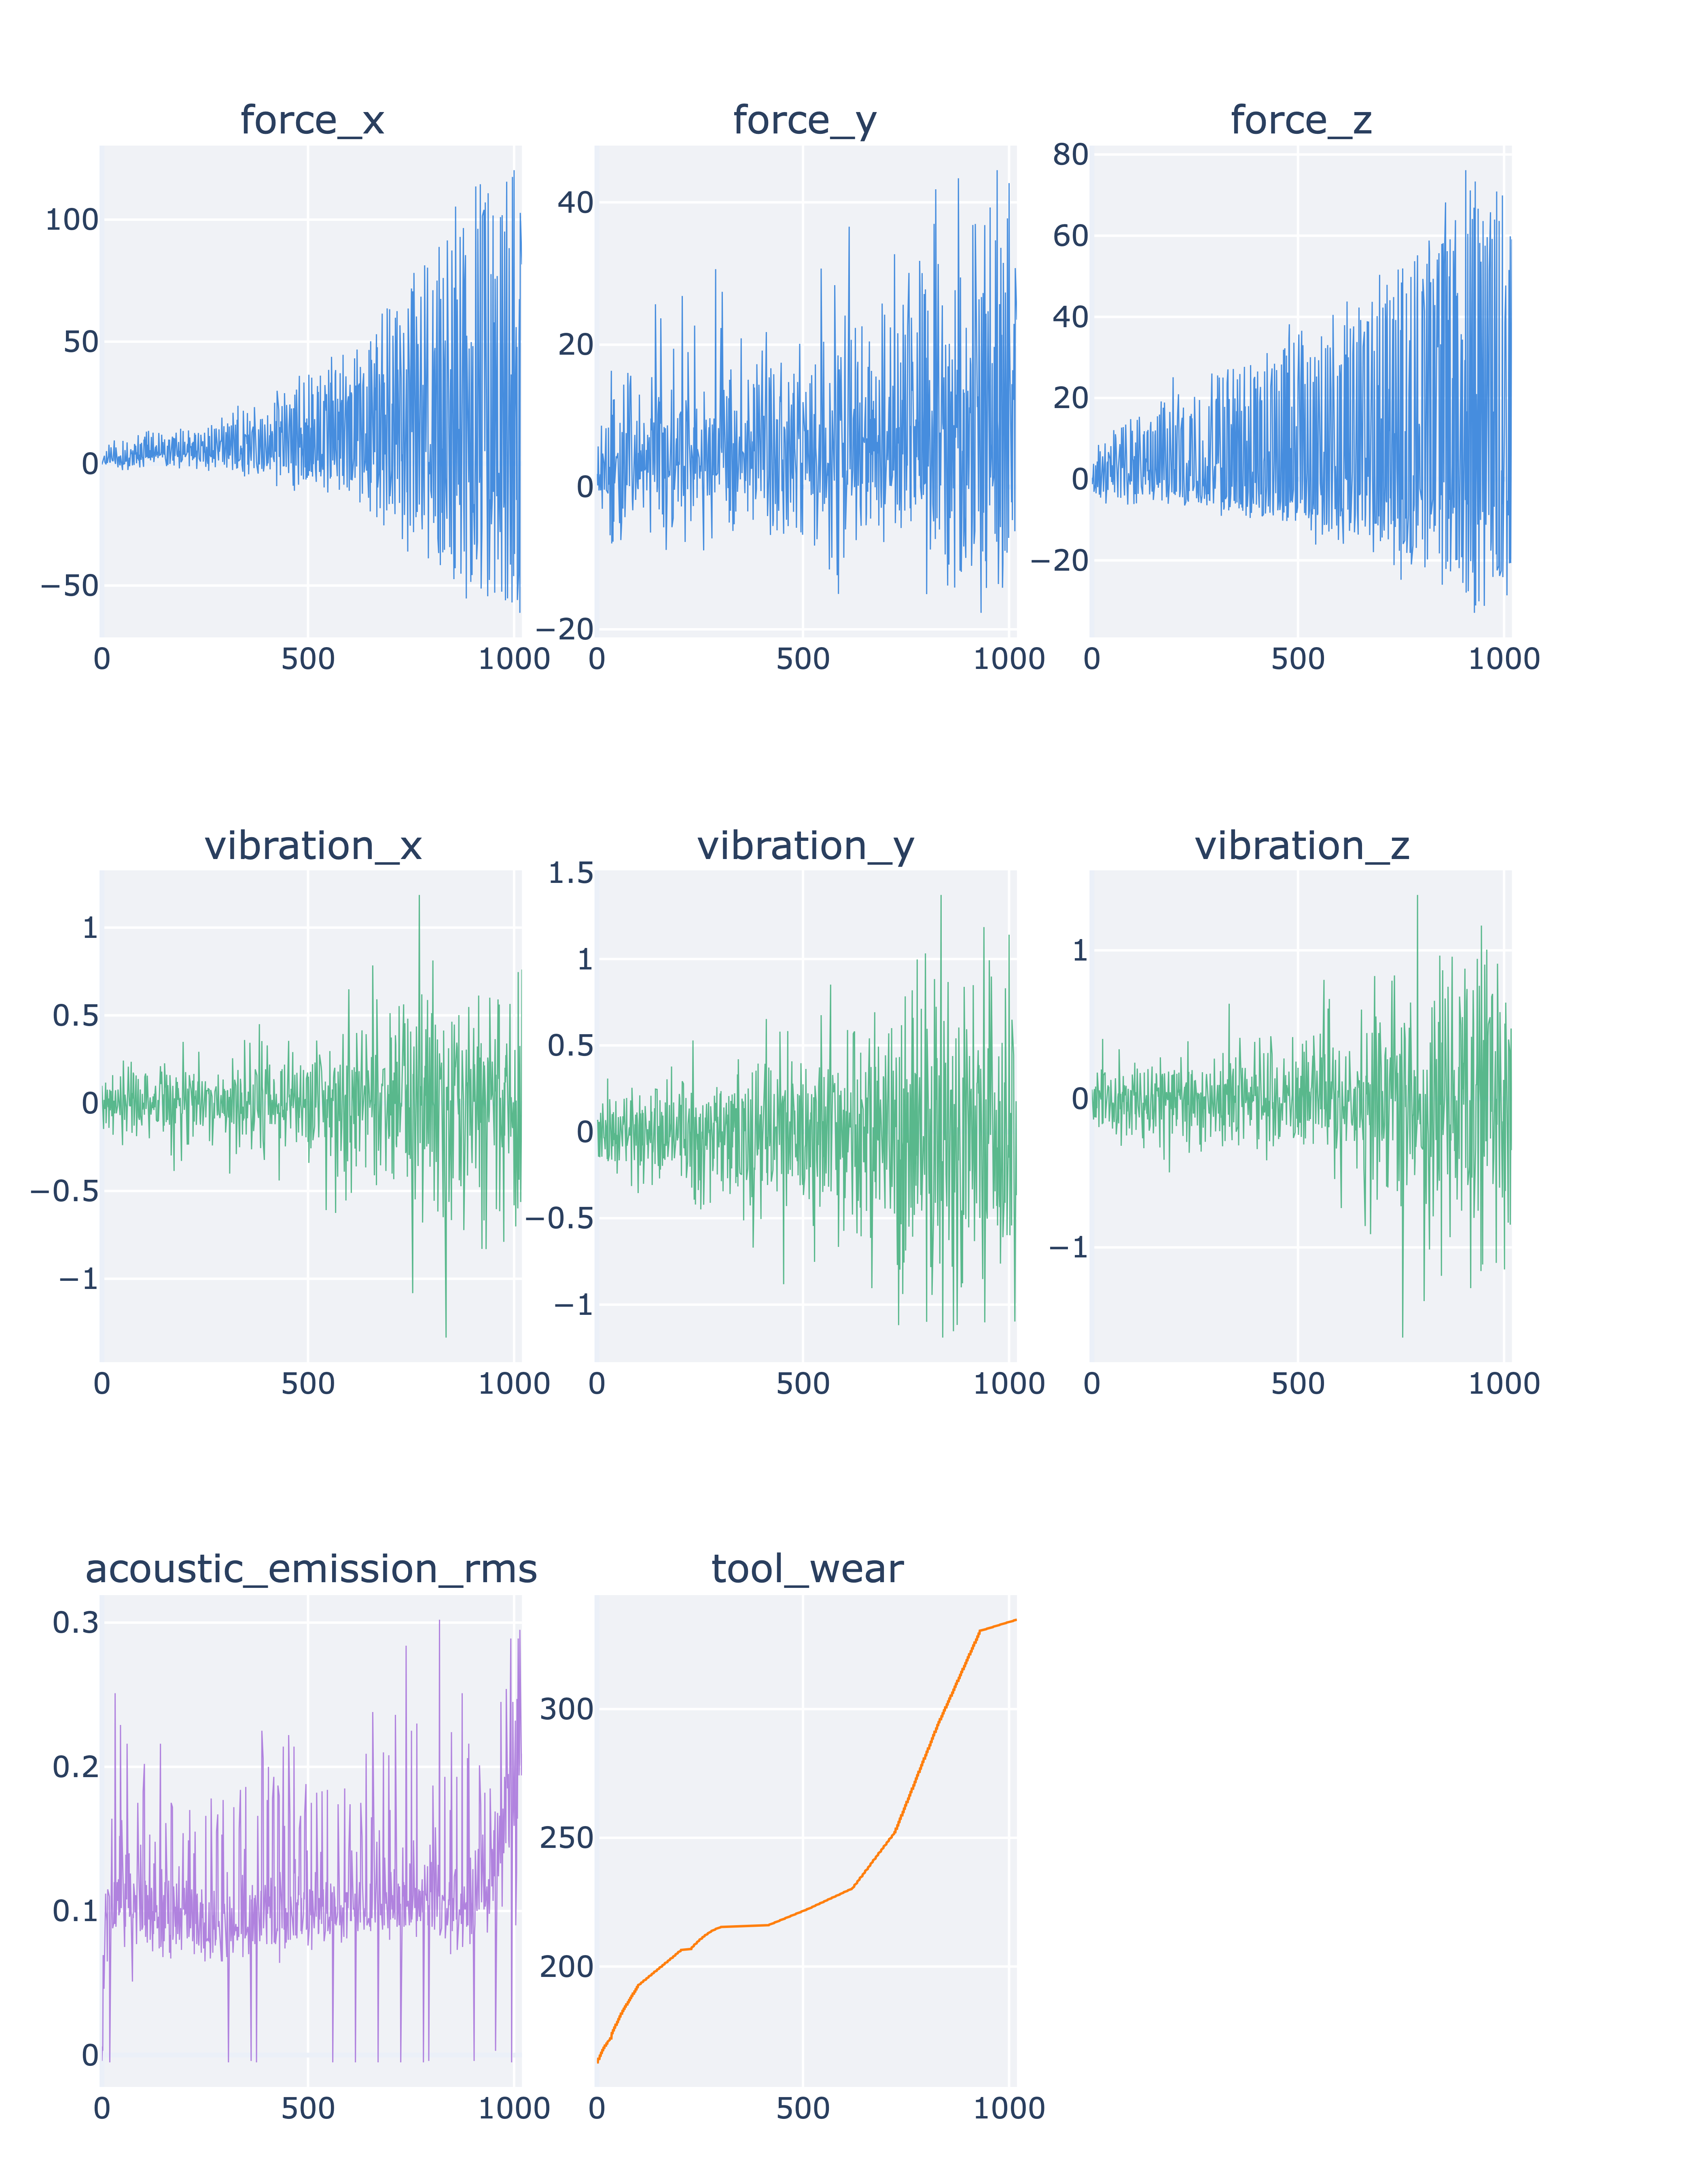
\includegraphics[width=\linewidth]{IEEE_06_SensorPlot.png}
		\caption{IEEE schema features.}
		\label{fig:schema_ieee}
	\end{subfigure}\hfill
	\begin{subfigure}[t]{0.48\textwidth}
		\centering
		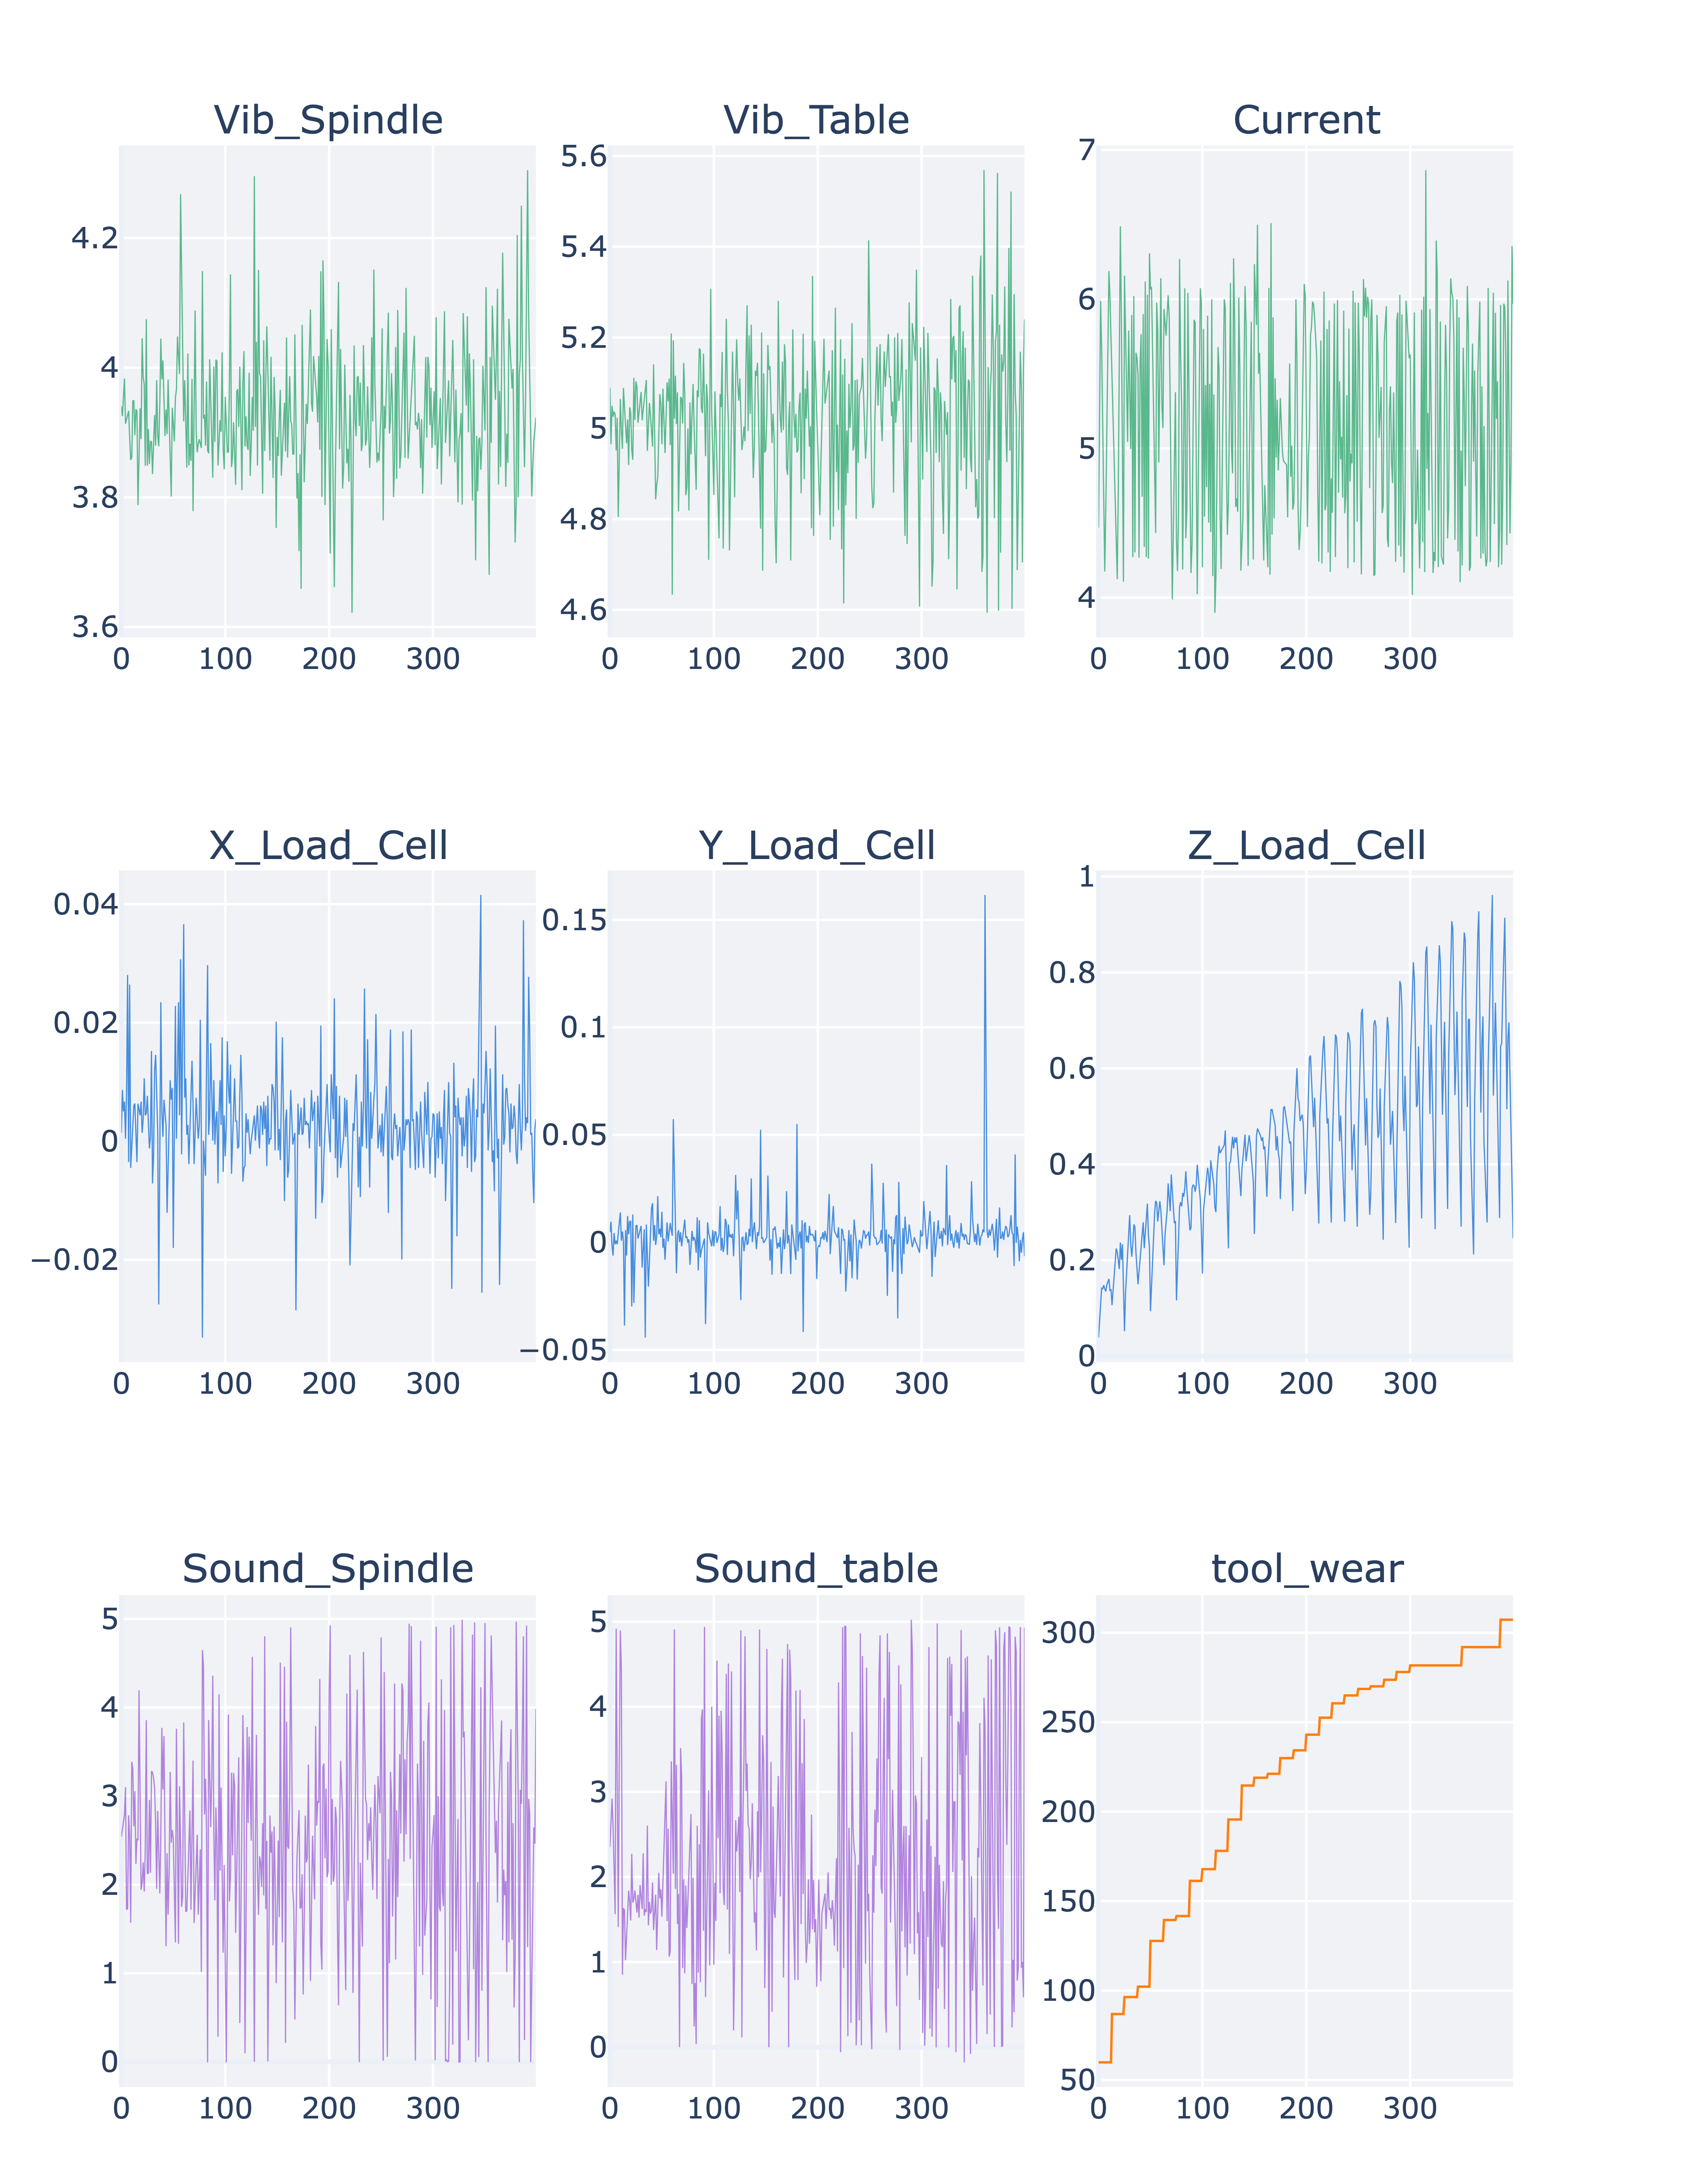
\includegraphics[width=\linewidth]{SIT_20_SensorPlot.png}
		\caption{SIT schema features.}
		\label{fig:schema_sit}
	\end{subfigure}

	\caption{IEEE and SIT schema feature plots: Representational plots depicting differences in sensor features, value ranges, and variations.}
	\label{fig:schema_feature_plots_ieee_sit}
\end{figure}

\begin{figure}[h]
	\centering
	\includegraphics[width=0.305\linewidth]{Expt_Setup_MillingMachine.png}
	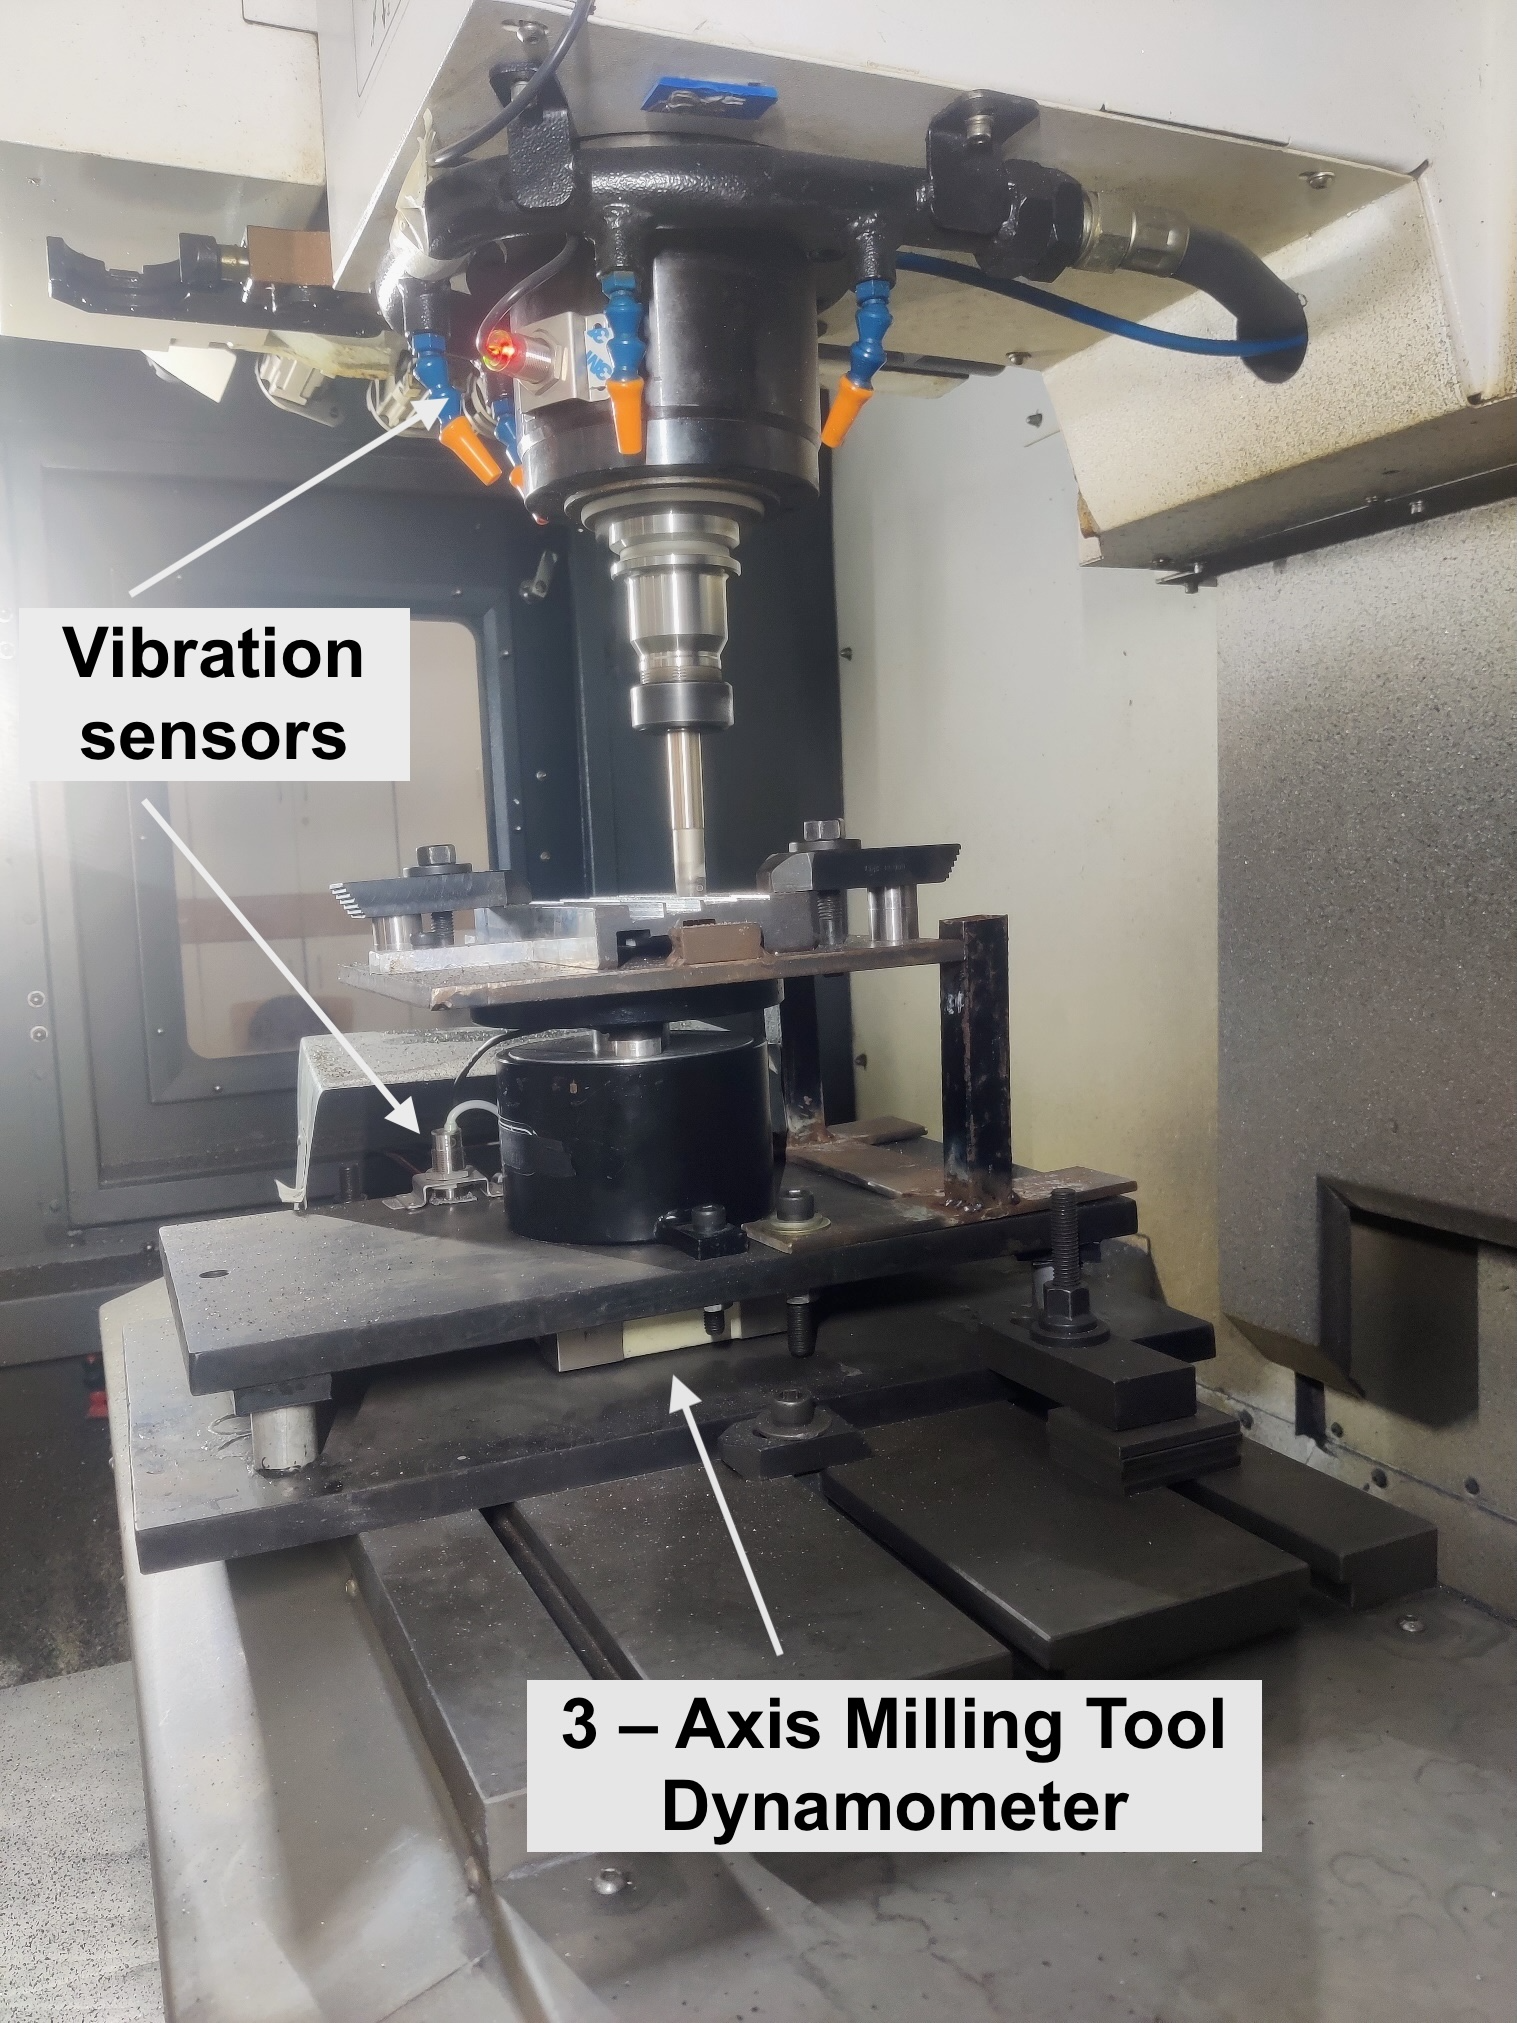
\includegraphics[width=0.45\linewidth]{Expt_Setup_Vibration_and_Dynamometer.png}
	\caption{Experimental setup - Machine and sensors}
	\label{fig:expt-setup-1}
\end{figure}

\begin{figure}[h]
	\centering
	\includegraphics[width=0.45\textwidth]{Expt_Setup_DACS.png}
	\includegraphics[width=0.445\textwidth]{Expt_Setup_Microscope.png}
	\caption{Experimental setups - Measurement instruments}
	\label{fig:expt-setup-2}
\end{figure}

\textbf{Schema heterogeneity and environment robustness:}
The two schemas differ in both dimensionality (7 vs. 8 channels) and sensing modality (force/vibration/acoustic emission vs. vibration/sound/load/current). This heterogeneity is intentional: the environment uses schema-specific observation feature sets while keeping the action semantics (replace vs. continue) and wear-threshold termination logic fixed.

\paragraph{Datasets and generalization protocol:}
The study uses two sensor schemas: (i) SIT (production-oriented schema with eight sensor channels), and (ii) IEEE (benchmark schema with force, vibration, and acoustic emission channels). Generalization is evaluated via a one-vs-all protocol: agents are trained on training file(s) within a schema and evaluated on remaining unseen datasets within the same schema.

\paragraph{Baselines and metrics:}
\label{sec:metrics}
The primary comparison in this paper is among RL agents that consume raw sensor observations directly. We do not include conventional supervised-ML baselines in this version because such pipelines typically require additional target construction, forecasting design choices, or task-specific feature engineering that vary substantially across schemas and practitioner settings. This omission should be treated as a scope choice rather than a claim that conventional ML is unsuitable; adding strong non-RL baselines remains an important extension for future work.

\paragraph{Evaluation metrics:}
We report three metrics used by the AutoRL evaluation: (i) evaluation score, (ii) tool usage (\%), and (iii) a $\lambda$ timing metric. Each trained model is evaluated for 20 stochastic rounds per test file.

\paragraph{Evaluation score definition:}
Let $u\in[0,1]$ be the tool-usage fraction at first replacement, let $v\in\mathbb{N}_0$ be the number of post-threshold timesteps without replacement (threshold violations), and let $\lambda$ be the signed timing error defined below. The evaluation score is
\begin{align}
S_{\text{tool}} &= u,\\
S_{\text{tim}} &= \max\left(0,\,1-\frac{|\lambda|}{c_{\mathrm{IAR}}}\right),\\
S_{\text{viol}} &= \frac{1}{1+v},\\
S &= 0.50\,S_{\text{tool}} + 0.30\,S_{\text{tim}} + 0.20\,S_{\text{viol}}.
\end{align}
Here $c_{\mathrm{IAR}}$ is a scaling constant (defined below) used only to map $\lambda$ to a unit interval for aggregation; it should be interpreted as the length of the in-advance replacement (IAR) window in timesteps.

%% Lambda
\paragraph{Lambda metric and offline prognostic evaluation:}
We implement a timing metric inspired by offline prognostic evaluation concepts \cite{Saxena2010Metrics}. Define $t_{\lambda}$ as the first timestep where wear exceeds an ``in-advance replacement'' (IAR) lower bound. Let $t_{\mathrm{FR}}$ be the first replacement timestep. Then
\begin{equation}
		\lambda = t_{\lambda} - t_{\mathrm{FR}}.
\end{equation}
Define $t_{\tau}$ as the first timestep where wear exceeds the wear threshold $\tau$. We set
\begin{equation}
\qquad c_{\mathrm{IAR}} = t_{\tau}-t_{\lambda},
\end{equation}
so that $S_{\text{tim}}$ linearly penalizes timing error over the IAR window and is clipped at zero outside that window.

\paragraph{Multi-round evaluation, confidence intervals, and hypothesis tests:}
Each trained model is evaluated for 20 rounds per held-out file to quantify variance from stochastic action sampling. Hypothesis testing uses one-tailed Welch $t$-tests at $\alpha=0.05$.

\textbf{Aggregation and 95\% confidence intervals:}
Let $S_1,\ldots,S_n$ denote the evaluation scores obtained across rounds and test files. We report the sample mean and standard deviation
\begin{align}
\mu &= \frac{1}{n}\sum_{i=1}^{n} S_i,\\
\sigma &= \sqrt{\frac{1}{n-1}\sum_{i=1}^{n}(S_i-\mu)^2},
\end{align}
and the standard error of the mean $\mathrm{SEM}=\sigma/\sqrt{n}$. A normal-approximation 95\% CI is then $[\mu-1.96\,\mathrm{SEM},\;\mu+1.96\,\mathrm{SEM}]$.

\section{Results} \label{sec:results}
This section reports consolidated evidence from the SIT and IEEE experiments under the same environment and evaluation protocol.

For each schema, we train four RL algorithms (\textsc{A2C}, \textsc{DQN}, \textsc{PPO}, \textsc{REINFORCE}) with four attention extractors (NW/TP/SA/MH) and evaluate each trained model for 20 stochastic rounds per held-out file.

\paragraph{Datasets:}
SIT uses 7 training files and 14 evaluation files (112 trained models total). IEEE uses 5 training files and 5 evaluation files (80 trained models total).

\subsection{Quantitative comparisons and statistical evidence}
\label{sec:hypothesis_tests}

The core quantitative evidence is reported in Tables~\ref{tab:hyp_tests}--\ref{tab:model_size_summary}.

Hypothesis test performed with one-tailed Welch $t$-tests at $\alpha=0.05$ for each schema. Table~\ref{tab:hyp_tests} summarizes the results under two categories - overall and using the best performing attention mechanism.

\begin{table}[htbp]
	\centering
	\caption{Pairwise comparison tests: one-tailed Welch $t$-tests comparing REINFORCE to each competitor at $\alpha=0.05$.}
	\label{tab:hyp_tests}
	\begin{tabular}{l l r r l}
	\toprule
	\textbf{Dataset} & \textbf{Competitor} & \textbf{t} & \textbf{p (1-tail)} & \textbf{Significance}\\
	\midrule
	\multicolumn{5}{l}{\textbf{Overall}}\\
	\faintcmidrule{1-5}
	\multirow{3}{*}{SIT}
		& A2C & 198.007 & 0.000 & Yes\\
		& DQN & 202.449 & 0.000 & Yes\\
		& PPO & 20.686 & 0.000 & Yes\\
	\faintcmidrule{1-5}
	\multirow{3}{*}{IEEE}
		& A2C & 10.726 & 0.000 & Yes\\
		& DQN & 15.977 & 0.000 & Yes\\
		& PPO & 1.957 & 0.026 & Yes\\
	\midrule
	\multicolumn{5}{l}{\textbf{Best attention mechanism}}\\
	\faintcmidrule{1-5}
	\multirow{3}{*}{SIT}
		& A2C & 512.423 & 0.000 & Yes\\
		& DQN & 562.313 & 0.000 & Yes\\
		& PPO & 49.902 & 0.000 & Yes\\
	\faintcmidrule{1-5}
	\multirow{3}{*}{IEEE}
		& A2C & 10.434 & 0.000 & Yes\\
		& DQN & 15.235 & 0.000 & Yes\\
		& PPO & 2.096 & 0.020 & Yes\\
	\bottomrule
	\end{tabular}
\end{table}

\paragraph{Hypothesis-driven interpretation (H1--H3):}
Let $S$ denote the evaluation score (Section~\ref{sec:metrics}). For each schema and competitor $c\in\{\textsc{A2C},\textsc{DQN},\textsc{PPO}\}$, Table~\ref{tab:hyp_tests} reports one-tailed Welch $t$-tests (at $\alpha=0.05$) for whether \textsc{REINFORCE} achieves a higher mean $S$ than $c$ under repeated stochastic evaluation.

Evaluations are performed on held out data and evaluation scores are computed per (model, held-out file) pair by averaging over the 20 stochastic rounds; reported $n$ values count these model--test-dataset pairs.

\textbf{H1 (primary): \textsc{REINFORCE} is competitive with A2C/DQN/PPO:}
All reported comparisons satisfy $p<0.05$ for both SIT and IEEE (Table~\ref{tab:hyp_tests}), providing evidence---under the adopted protocol---that \textsc{REINFORCE} achieves higher mean scores than \textsc{A2C} and \textsc{DQN} on both schemas and is close to (but statistically above) \textsc{PPO}. The IEEE \textsc{PPO} comparison is the tightest (overall: $t=1.957$, $p=0.026$), consistent with near-ties in mean-score summaries.

\textbf{H2: schema portability of environment and reward logic:}
H2 is supported by the cross-schema consistency of the hypothesis-test outcomes: the same environment design and reward shaping yield a stable ranking signal in both SIT and IEEE, with \textsc{REINFORCE} significantly outperforming \textsc{A2C} and \textsc{DQN} and remaining close to (but still statistically above) \textsc{PPO}. This should be interpreted as \emph{schema portability} of the experimental pipeline and MDP formulation---i.e., the same formulation produces meaningful learning and evaluation behaviour across heterogeneous sensor schemas---not as direct transfer of a trained policy from one schema to the other.

\textbf{H3: attention mechanisms improve \textsc{REINFORCE} performance:}
We do not include a no-attention ablation in this grid, so H3 is supported indirectly: (i) \textsc{REINFORCE} performance varies materially across attention extractors, and (ii) the best-performing \textsc{REINFORCE} configurations in both schemas use attention (Tables~\ref{tab:sit_top10} and \ref{tab:ieee_top10}).


\paragraph{Visual summaries using analysis dashboards}
Figure~\ref{fig:analysis_sit} and Figure~\ref{fig:analysis_ieee} provide consolidated dashboards for each schema. Figure~\ref{fig:heatmap_sit} and Figure~\ref{fig:heatmap_ieee} complement these dashboards with one-vs-all generalization heatmaps.

\begin{figure}[t]
	\centering
	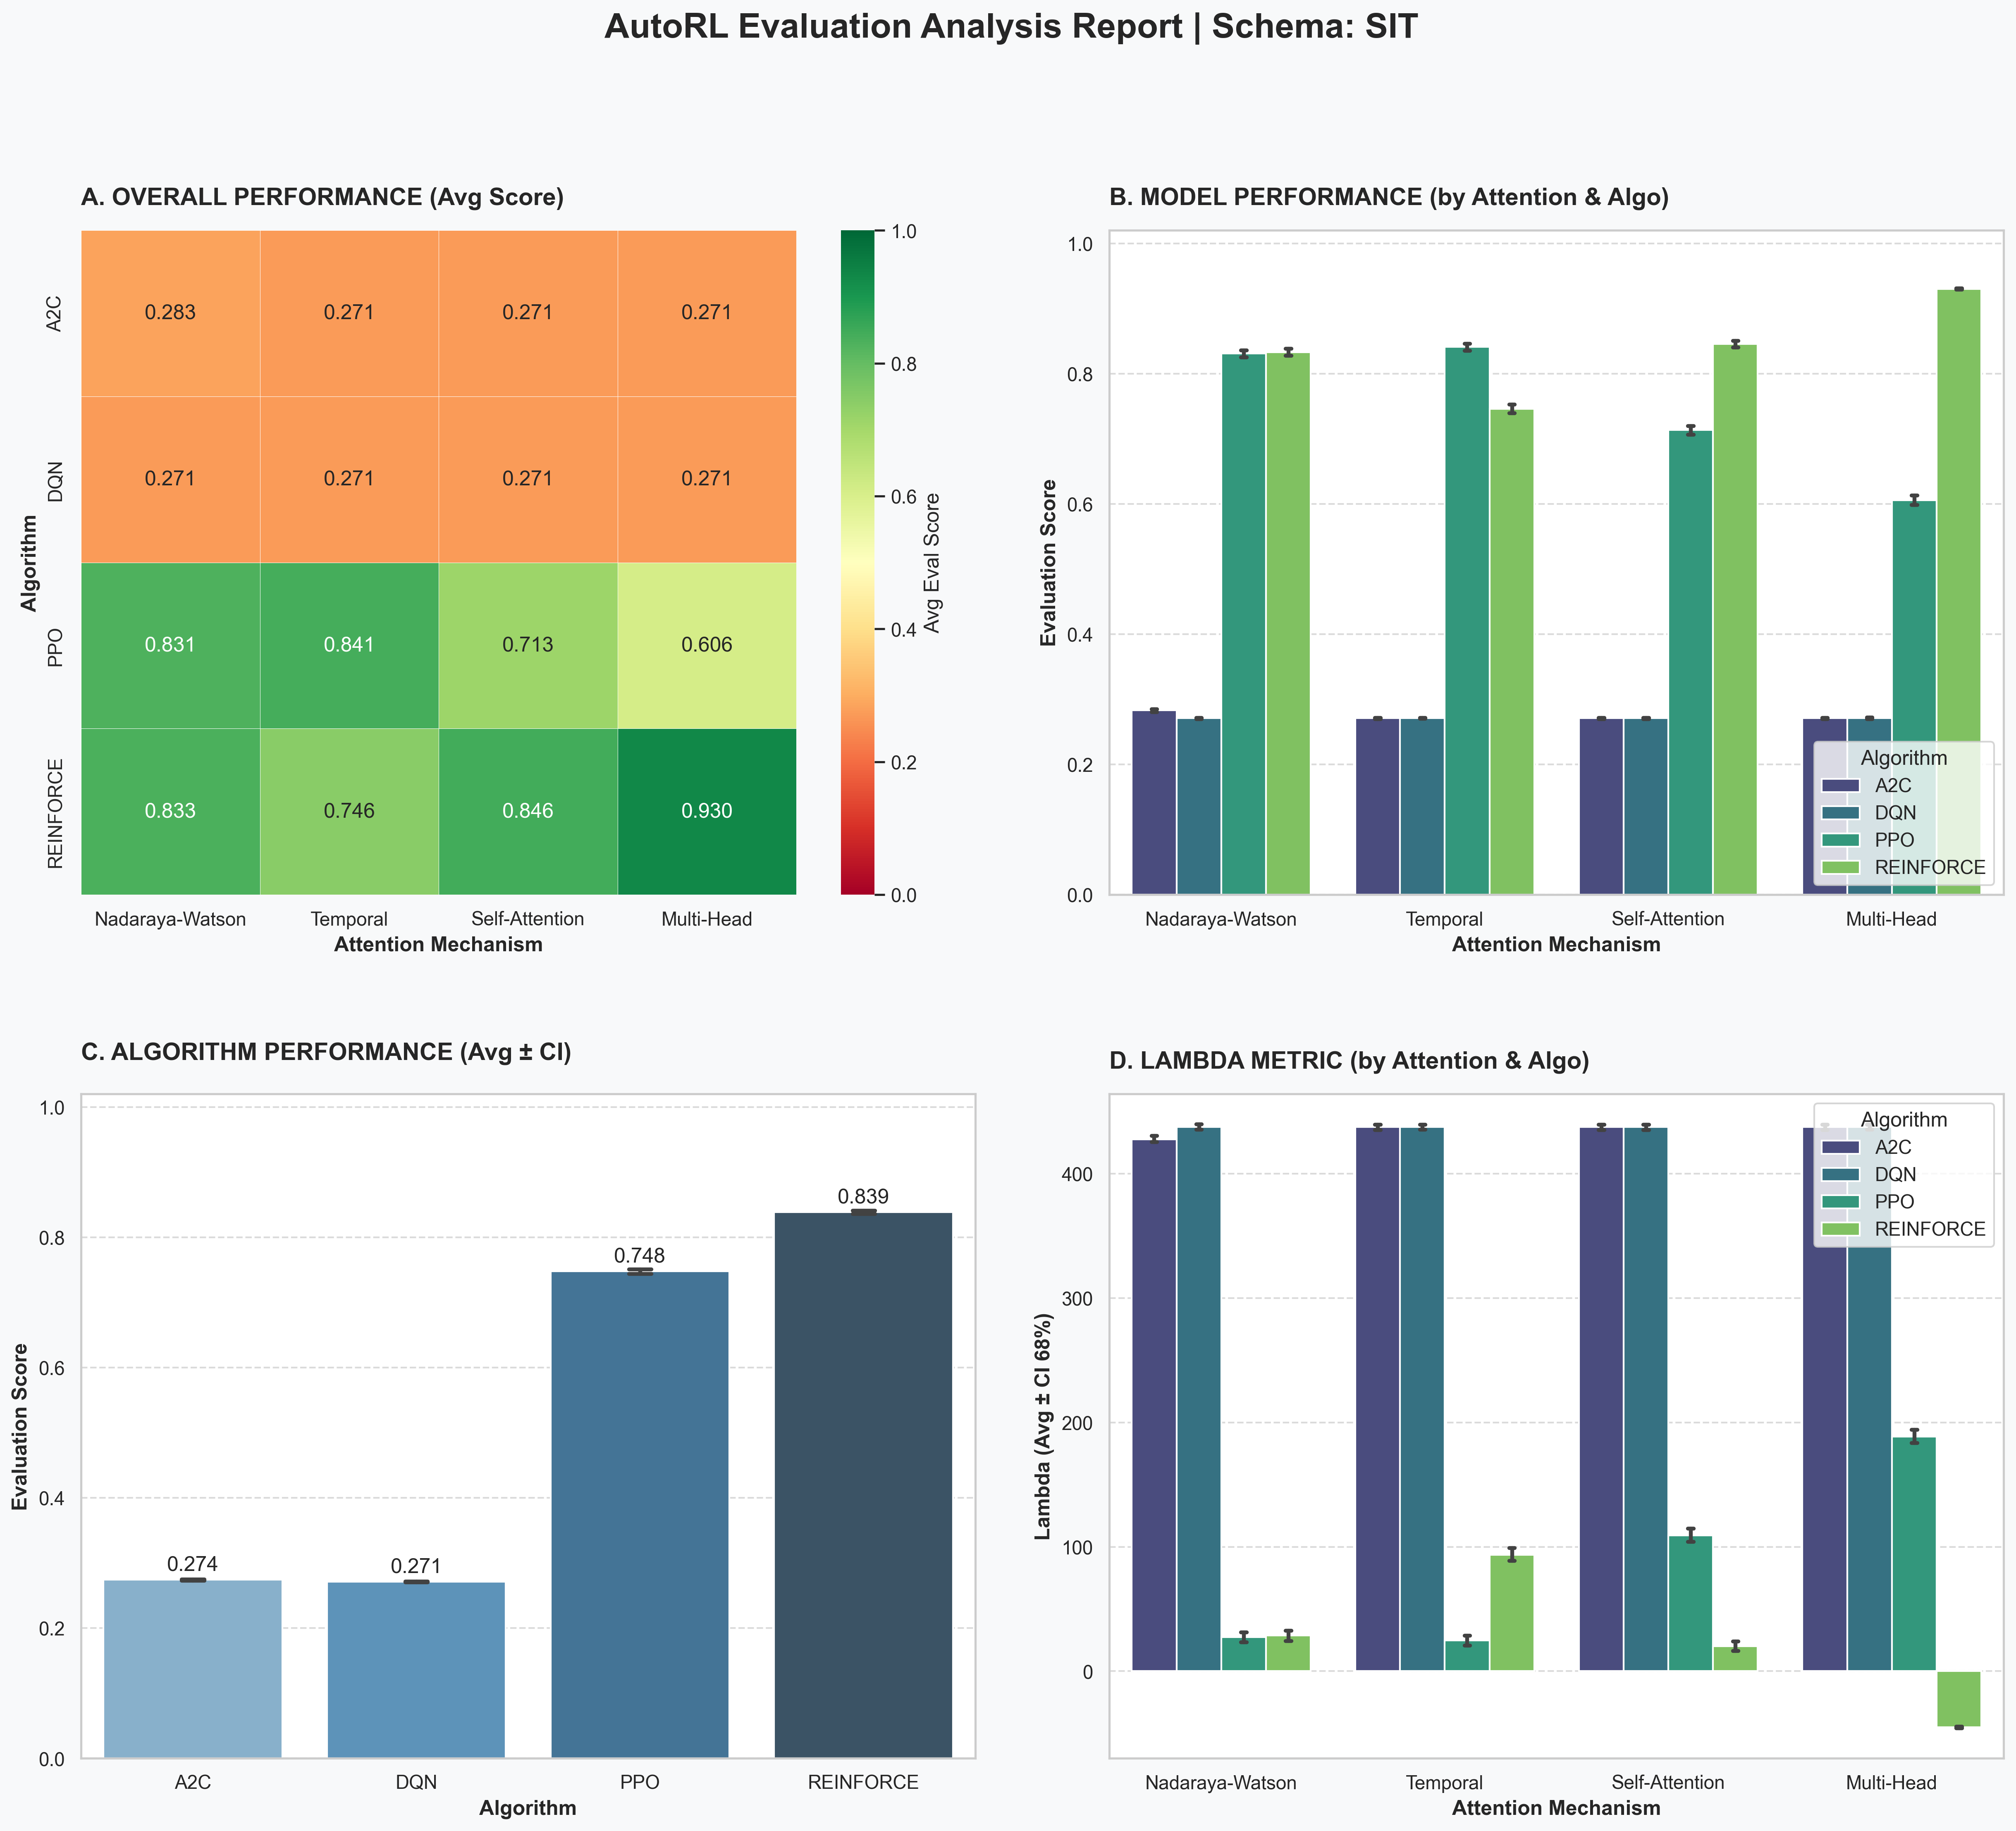
\includegraphics[width=0.95\textwidth]{_Analysis_Report_SIT.png}
	\caption{Consolidated evaluation dashboard for SIT (mean and uncertainty/error bars) used as primary visual evidence for performance patterns across algorithms and attention mechanisms.}
	\label{fig:analysis_sit}
\end{figure}

\begin{figure}[t]
	\centering
	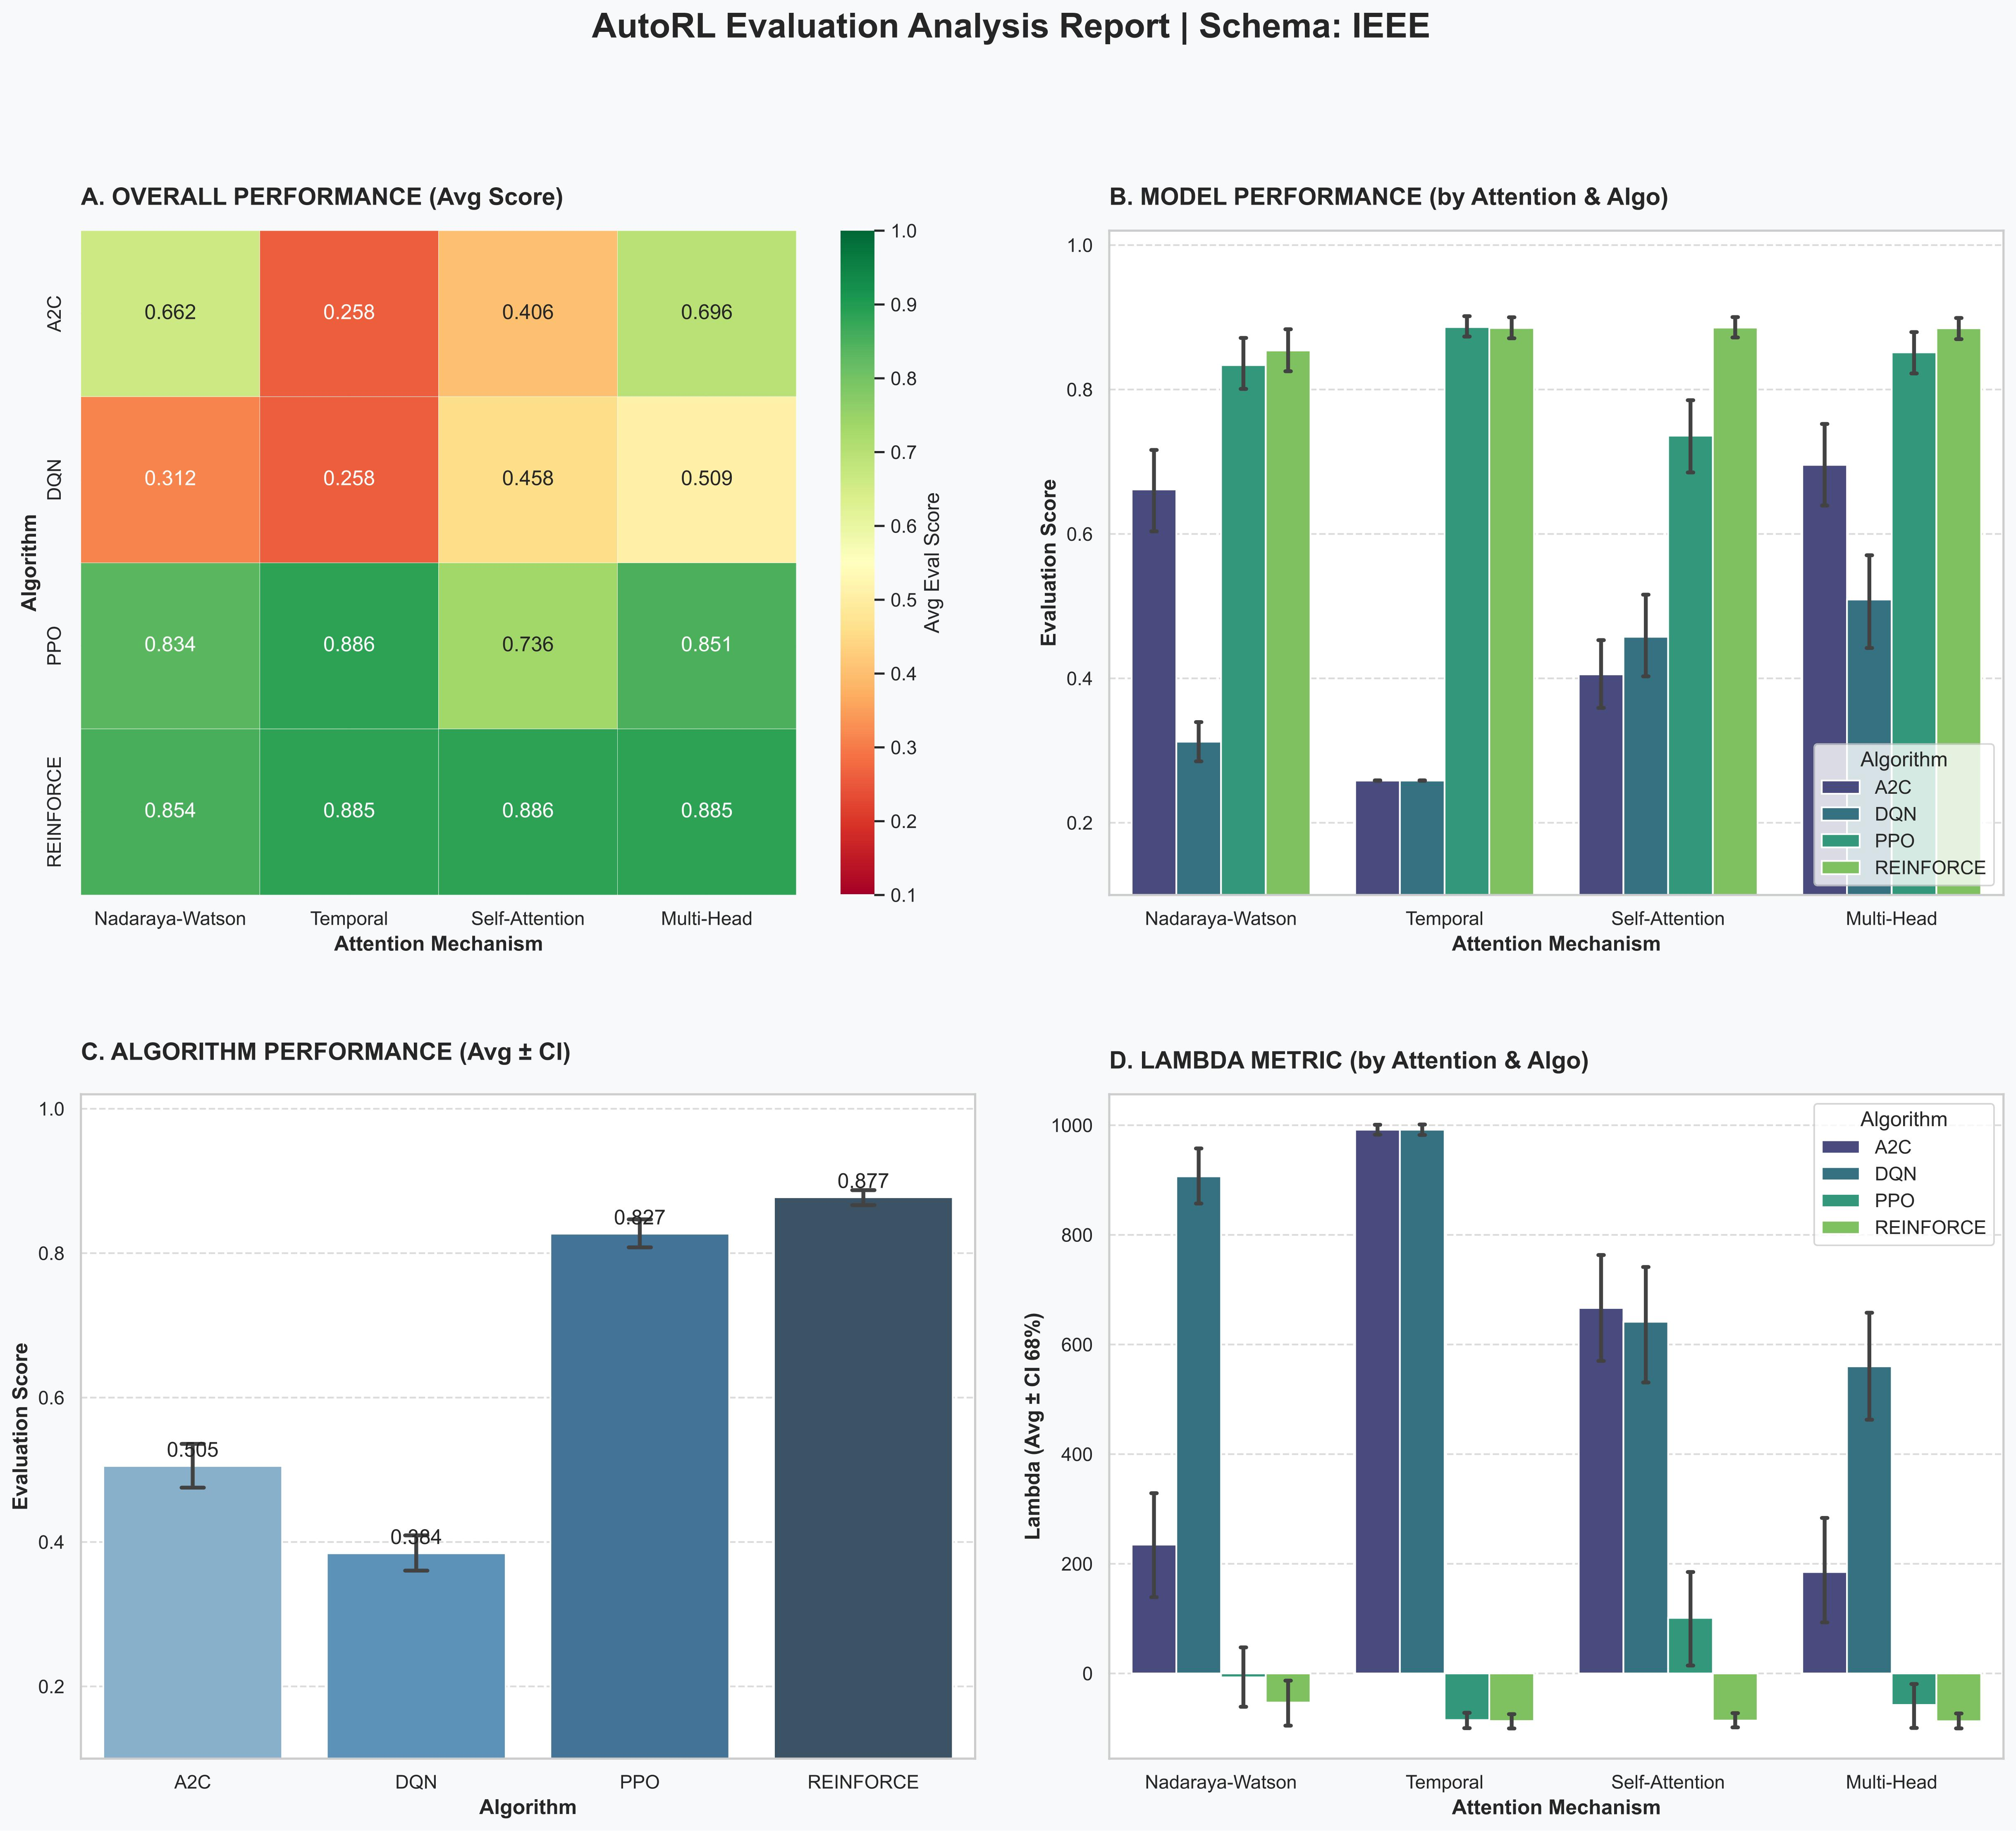
\includegraphics[width=0.95\textwidth]{_Analysis_Report_IEEE.jpg}
	\caption{Consolidated evaluation dashboard for IEEE (mean and uncertainty/error bars) used as primary visual evidence for performance patterns across algorithms and attention mechanisms.}
	\label{fig:analysis_ieee}
\end{figure}

\paragraph{Quantitative summaries (means and 95\% CI):}
Tables~\ref{tab:sit_top10} and \ref{tab:ieee_top10} list the top configurations by mean evaluation score. Tables~\ref{tab:sit_best_attn} and \ref{tab:ieee_best_attn} summarize the best attention mechanism per algorithm.

\begin{table}
\caption{Top 5 SIT models by mean evaluation score (aggregated across trained models and held-out files)}
\label{tab:sit_top10}
\begin{tabular}{ll r r r r}
\toprule
\textbf{Algorithm} & \textbf{Attention} & \textbf{Eval. Score} & \textbf{95\% CI} & \textbf{Tool use (\%)} & \textbf{$\lambda$}\\
\midrule
    \textbf{REINFORCE} & \textbf{Multi-Head} & \textbf{0.930} & \textbf{0.002} & \textbf{96.637} & \textbf{-45.020} \\
    REINFORCE & Self-Attention & 0.846 & 0.010 & 90.733 & 20.041 \\
    PPO & Temporal & 0.841 & 0.010 & 90.288 & 24.878 \\
    REINFORCE & Nadaraya-Watson & 0.833 & 0.011 & 89.768 & 28.571 \\
    PPO & Nadaraya-Watson & 0.831 & 0.011 & 89.862 & 27.520 \\
    \bottomrule
\end{tabular}
\end{table}


\begin{table}[htbp]
	\centering
	\caption{Top 5 IEEE models by mean evaluation score (aggregated across trained models and held-out files)}
	\label{tab:ieee_top10}
	\begin{tabular}{ll r r r r}
	\toprule
	\textbf{Algorithm} & \textbf{Attention} & \textbf{Eval. Score} & \textbf{95\% CI} & \textbf{Tool use (\%)} & \textbf{$\lambda$}\\
	\midrule
	\textbf{REINFORCE} & \textbf{Multi-Head} & \textbf{0.886} & \textbf{0.031} & \textbf{95.215} & \textbf{-85.700}\\
	REINFORCE & Self-Attention 	& 0.886 & 0.031 & 95.261 & -86.100\\
	PPO & Temporal 				& 0.886 & 0.031 & 95.199 & -85.050\\
	REINFORCE & Temporal 		& 0.885 & 0.031 & 95.341 & -86.750\\
	PPO & Nadaraya-Watson 	& 0.857 & 0.070 & 93.651 & -31.900\\
	\bottomrule
	\end{tabular}
\end{table}


\begin{table}
	\caption{SIT: Algorithms with best performing attention mechanism.}
	\label{tab:sit_best_attn}
	\begin{tabular}{l l r r r}
	\toprule
	\textbf{Algorithm} & \textbf{Best attention} & \textbf{Eval. Score} & \textbf{CI} & \textbf{n}\\
	\midrule
		A2C & Nadaraya-Watson & 0.283 & 0.004 & 1568 \\
		DQN & Multi-Head & 0.271 & 0.002 & 1568 \\
		PPO & Temporal & 0.841 & 0.010 & 1568 \\
		\textbf{REINFORCE} & \textbf{Multi-Head} & \textbf{0.930} & \textbf{0.002} & 1568 \\
	\bottomrule
	\end{tabular}
\end{table}

\begin{table}[htbp]
	\centering
	\caption{IEEE: Algorithms with best performing attention mechanism.}
	\label{tab:ieee_best_attn}
	\begin{tabular}{l l r r r}
	\toprule
	\textbf{Algorithm} & \textbf{Best attention} & \textbf{Eval. Score} & \textbf{CI} & \textbf{n}\\
	\midrule
		A2C & Multi-Head & 0.696 & 0.113 & 400 \\
		DQN & Multi-Head & 0.509 & 0.124 & 400 \\
		PPO & Temporal & 0.886 & 0.028 & 400 \\
		\textbf{REINFORCE} & \textbf{Self-Attention} & \textbf{0.886} & \textbf{0.021} & 400 \\
	\bottomrule
	\end{tabular}
\end{table}

\paragraph{Model footprint (serialized sizes):} 
Table~\ref{tab:model_size_summary} summarizes per-algorithm average serialized sizes. Table~\ref{tab:deep_edge_mcus} show common industrial edge computing MCUs (microcontrollers). MCU memory size must hold the model, configuration files, allow run-time memory and free memory to run the inferences. This implies any models less than 256 kB will allow robust operations. With the lowest size REINFORCE demonstrates it is a candidate for edge devices.

\begin{table}[htbp]
\centering
\caption{Average serialized policy size (kB), averaged over models within each schema.}
\label{tab:model_size_summary}
\begin{tabular}{l r r}
\toprule
	\textbf{Algorithm} & \textbf{SIT avg. (kB)} & \textbf{IEEE avg. (kB)}\\
	\midrule
	A2C & 293.55 & 292.54\\
	DQN & 419.73 & 417.72\\
	PPO & 169.90 & 169.38\\
	\textbf{REINFORCE} & \textbf{169.47} & \textbf{168.95}\\
\bottomrule
\end{tabular}
\end{table}

\subsection{Schema portability and attention sensitivity}
\textbf{Dataset-level interpretation:}
\textbf{SIT (consolidated):} SIT results show a clear separation between the two lightweight baselines (A2C/DQN) and the two top performers (PPO/\textsc{REINFORCE}) across attention mechanisms.

\textbf{IEEE:} IEEE results show a tighter competition between PPO and \textsc{REINFORCE}. The best configurations are effectively tied at the reported precision: PPO with temporal attention and \textsc{REINFORCE} with multi-head or self-attention all achieve mean evaluation scores of about 0.886 (Tables~\ref{tab:ieee_top10}--\ref{tab:ieee_best_attn}).

\textbf{Attention effects under H3:}
Attention improves \textsc{REINFORCE}, but no single mechanism dominates across both schemas. On SIT, multi-head attention is the clearest winner and yields the strongest overall \textsc{REINFORCE} configuration. On IEEE, multi-head, self-attention, and temporal attention are all strong, with only marginal differences at the reported precision.

\textbf{Practical recommendation:}
For edge-first deployments with constrained training and inference budgets, \emph{REINFORCE + Multi-Head attention} is a reasonable default for SIT-like settings. For IEEE-like settings, \textsc{REINFORCE}+multi-head, \textsc{REINFORCE}+self-attention, \textsc{REINFORCE}+temporal attention, and PPO+temporal attention appear closely matched.

\paragraph{H2: schema portability (SIT vs IEEE):}
H2 is supported structurally by the environment design (Section~\ref{sec:env}) and empirically by consistent learning and ranking signals on both schemas (Tables~\ref{tab:hyp_tests}--\ref{tab:ieee_best_attn}). This is best described as \emph{schema portability} of the environment formulation, not direct cross-schema transfer.

\section{Discussion}
\label{sec:discussion}
\subsection{Why lightweight REINFORCE can be competitive in this PdM setup}
The PdM task studied here has a small action space and terminates on replacement, but the policy still has to infer replacement timing from multivariate sensor trajectories rather than from direct inspection measurements. In such settings, representation quality can matter at least as much as optimizer sophistication; this helps explain why a lightweight policy-gradient method paired with suitable feature extraction can compete with heavier baselines.

\subsection{Implications for industrial practitioners and edge deployment}
The primary practical implication is that a lightweight policy-gradient learner (\textsc{REINFORCE}), when paired with appropriate attention-based feature extraction, is a viable option for edge-first PdM deployments where model footprint and operational simplicity matter. AutoRL serves as a standardized workflow that automates algorithm and attention sweeps and produces comparable result summaries for selection and auditing. A further practical advantage is that the RL agents in this study operate directly on raw sensor observations; by contrast, conventional ML alternatives often require additional feature engineering, target-construction choices, or domain-specific prognostics pipelines.

\paragraph{Edge compute and sustainability framing:}
This paper does not directly measure energy, latency, or memory on target edge hardware, so compute-efficiency is treated as a deployment motivation rather than an empirically validated claim. A practical design principle is to prefer the least complex method that meets the operational objective \cite{Schwartz2020, Strubell2019}.

\section{Conclusion}
\label{sec:conclusion}
\subsection{Summary of key findings}
This paper presented an empirical study of \textsc{REINFORCE} with attention mechanisms for milling-machine tool-replacement PdM under edge-oriented constraints. Using a schema-adaptive Gymnasium environment and multi-round evaluation on unseen data, the results indicate a consistent pattern across SIT and IEEE schemas: under the adopted evaluation protocol, \textsc{REINFORCE} emerges as a strong lightweight baseline, performing more strongly than \textsc{A2C} and \textsc{DQN} while remaining comparable to \textsc{PPO}. The study also shows that the same environment formulation and reward logic can be reused effectively across two materially different sensor schemas. Finally, attention is beneficial for \textsc{REINFORCE}, although the most effective choice is schema-dependent: multi-head attention is strongest on SIT, whereas several attention variants perform similarly on IEEE. Interpreted as representation-learning priors, the attention mechanisms bias the policy toward informative sensor patterns in an online monitoring setting.

\subsection{Future work}
Some limitations of our research could be addressed by future work and should (i) measure inference latency, serialized model size, and energy on representative edge devices, (ii) incorporate richer maintenance costs and state-estimation models, (iii) add non-RL baselines that operate on the same raw or minimally processed sensor streams, and (iv) evaluate robustness under sensor drift and cross-machine domain shift.


\section*{Acknowledgements}
The authors thank the anonymous reviewers and colleagues for feedback.

\section*{Declarations}

\subsection*{Funding}
The authors received no specific funding for this work.

\subsection*{Conflict of interest/Competing interests}
Not applicable

\subsection*{Ethics approval and consent to participate}
Not applicable

\subsection*{Consent for publication}
Not applicable

\subsection*{Data availability}
The IEEE PHM~2010 milling dataset is publicly available \cite{PHMdata2010}. The SIT dataset used in this study contains in-house experimental measurements and is available from the corresponding author upon reasonable request.

\subsection*{Materials availability}
Not applicable

\subsection*{Code availability}
The code used to train and evaluate the agents (AutoRL pipeline and the Gymnasium environment) is available from the authors upon reasonable request.

\subsection*{Author contribution}
\begin{itemize}
	\item Conceptualization: Rajesh Siraskar, Satish Kumar
	\item Methodology: Rajesh Siraskar, Satish Kumar, Shruti Patil
	\item Milling machine set-up and data gathering:  
\end{itemize}

\begin{appendices}

\section{Edge deployment context}\label{app:edge_context}

\begin{table}[htbp]
	\centering
	\caption{Deep edge microcontrollers for predictive maintenance (256~kB to 2~MB SRAM)}
	\label{tab:deep_edge_mcus}
	\renewcommand{\arraystretch}{1.3}
	\begin{tabular}{@{} l l l l p{5.5cm} @{}}
		\toprule
		\textbf{MCU name} & \textbf{Architecture} & \textbf{Processor} & \textbf{Memory} & \textbf{Notes} \\
		\midrule
		STM32H7 series & ARM & Dual-core Cortex-M7 + M4 & Up to 2~MB & Industrial-grade; M7 handles ML math while M4 can handle real-time sensor control. \\
		NXP i.MX RT series & ARM & Cortex-M7 (up to 1~GHz) & 1~MB--2~MB & ``Crossover'' MCU; high clock speeds for heavier local analytics. \\
		Espressif ESP32-S3 & Xtensa & Dual-core LX7 & 512~kB & Built-in Wi-Fi/BLE.\\
		Nordic nRF5340 & ARM & Dual-core Cortex-M33 & 512~kB & Low-power BLE; separate cores for application and wireless stack. \\
		Renesas RA6M5 & ARM & Cortex-M33 & 512~kB & Industrial control focus; security and common industrial interfaces. \\
		Raspberry Pi RP2040 & ARM & Dual-core Cortex-M0+ & 264~kB & Cost-effective; Programmable I/O for custom sensor interfacing. \\
		Nordic nRF52840 & ARM & Cortex-M4F & 256~kB & Includes FPU; common in battery-operated nodes. \\
		\bottomrule
	\end{tabular}
\end{table}

\section{Progressive tool wear images - Samples}
\begin{table}[h!]
	\centering
	\caption{Progressive tool wear. Images taken using tool-makers microscope}
	\label{tab:wearimages}
	\begin{tabular}{|r|r|c|}
	\hline
	Runs & Wear $VB_{max}\mu$m & Tool condition\\
	\hline
	 0 &   0.00 & 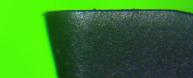
\includegraphics[width=0.3\linewidth]{tw-1.jpg} \\ \hline
	 5 & 119.71 & 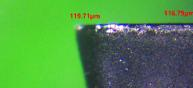
\includegraphics[width=0.3\linewidth]{tw-2.jpg} \\ \hline
	10 & 170.07 & 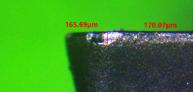
\includegraphics[width=0.3\linewidth]{tw-3.jpg} \\ \hline
	15 & 212.21 & 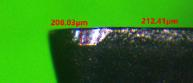
\includegraphics[width=0.3\linewidth]{tw-4.jpg} \\ \hline
	20 & 236.50 & 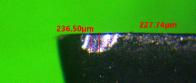
\includegraphics[width=0.3\linewidth]{tw-5.jpg} \\ \hline
	25 & 254.74 & 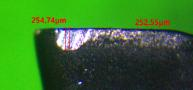
\includegraphics[width=0.3\linewidth]{tw-6.jpg} \\ \hline
	30 & 280.29 & 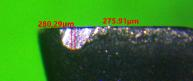
\includegraphics[width=0.3\linewidth]{tw-7.jpg} \\ \hline
	35 & 303.65 & 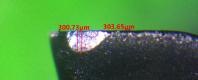
\includegraphics[width=0.3\linewidth]{tw-8.jpg} \\ \hline
	\end{tabular}
\end{table}

\end{appendices}

\bibliography{JoIM_references}

\end{document}

